% ============================================================
%  existing_solution.tex
%  Annotated screenshot of the eVici Produktliste UI.
%  Compile with: pdflatex existing_solution.tex
% ============================================================

\documentclass[tikz, border=5pt]{standalone}
\usepackage{tikz}
\usetikzlibrary{arrows.meta, calc, positioning, backgrounds, shadows}
\usepackage{lmodern}
\usepackage{graphicx}
\usepackage{xcolor}

% ---- Brand colours ----------------------------------------
\definecolor{strandOrange}{HTML}{E87722}
\definecolor{uiBorder}{HTML}{D1D5DB}

\begin{document}

\begin{tikzpicture}

  % --- Base screenshot -------------------------------------
  \node[anchor=south west, inner sep=0] (img) at (0,0)
      {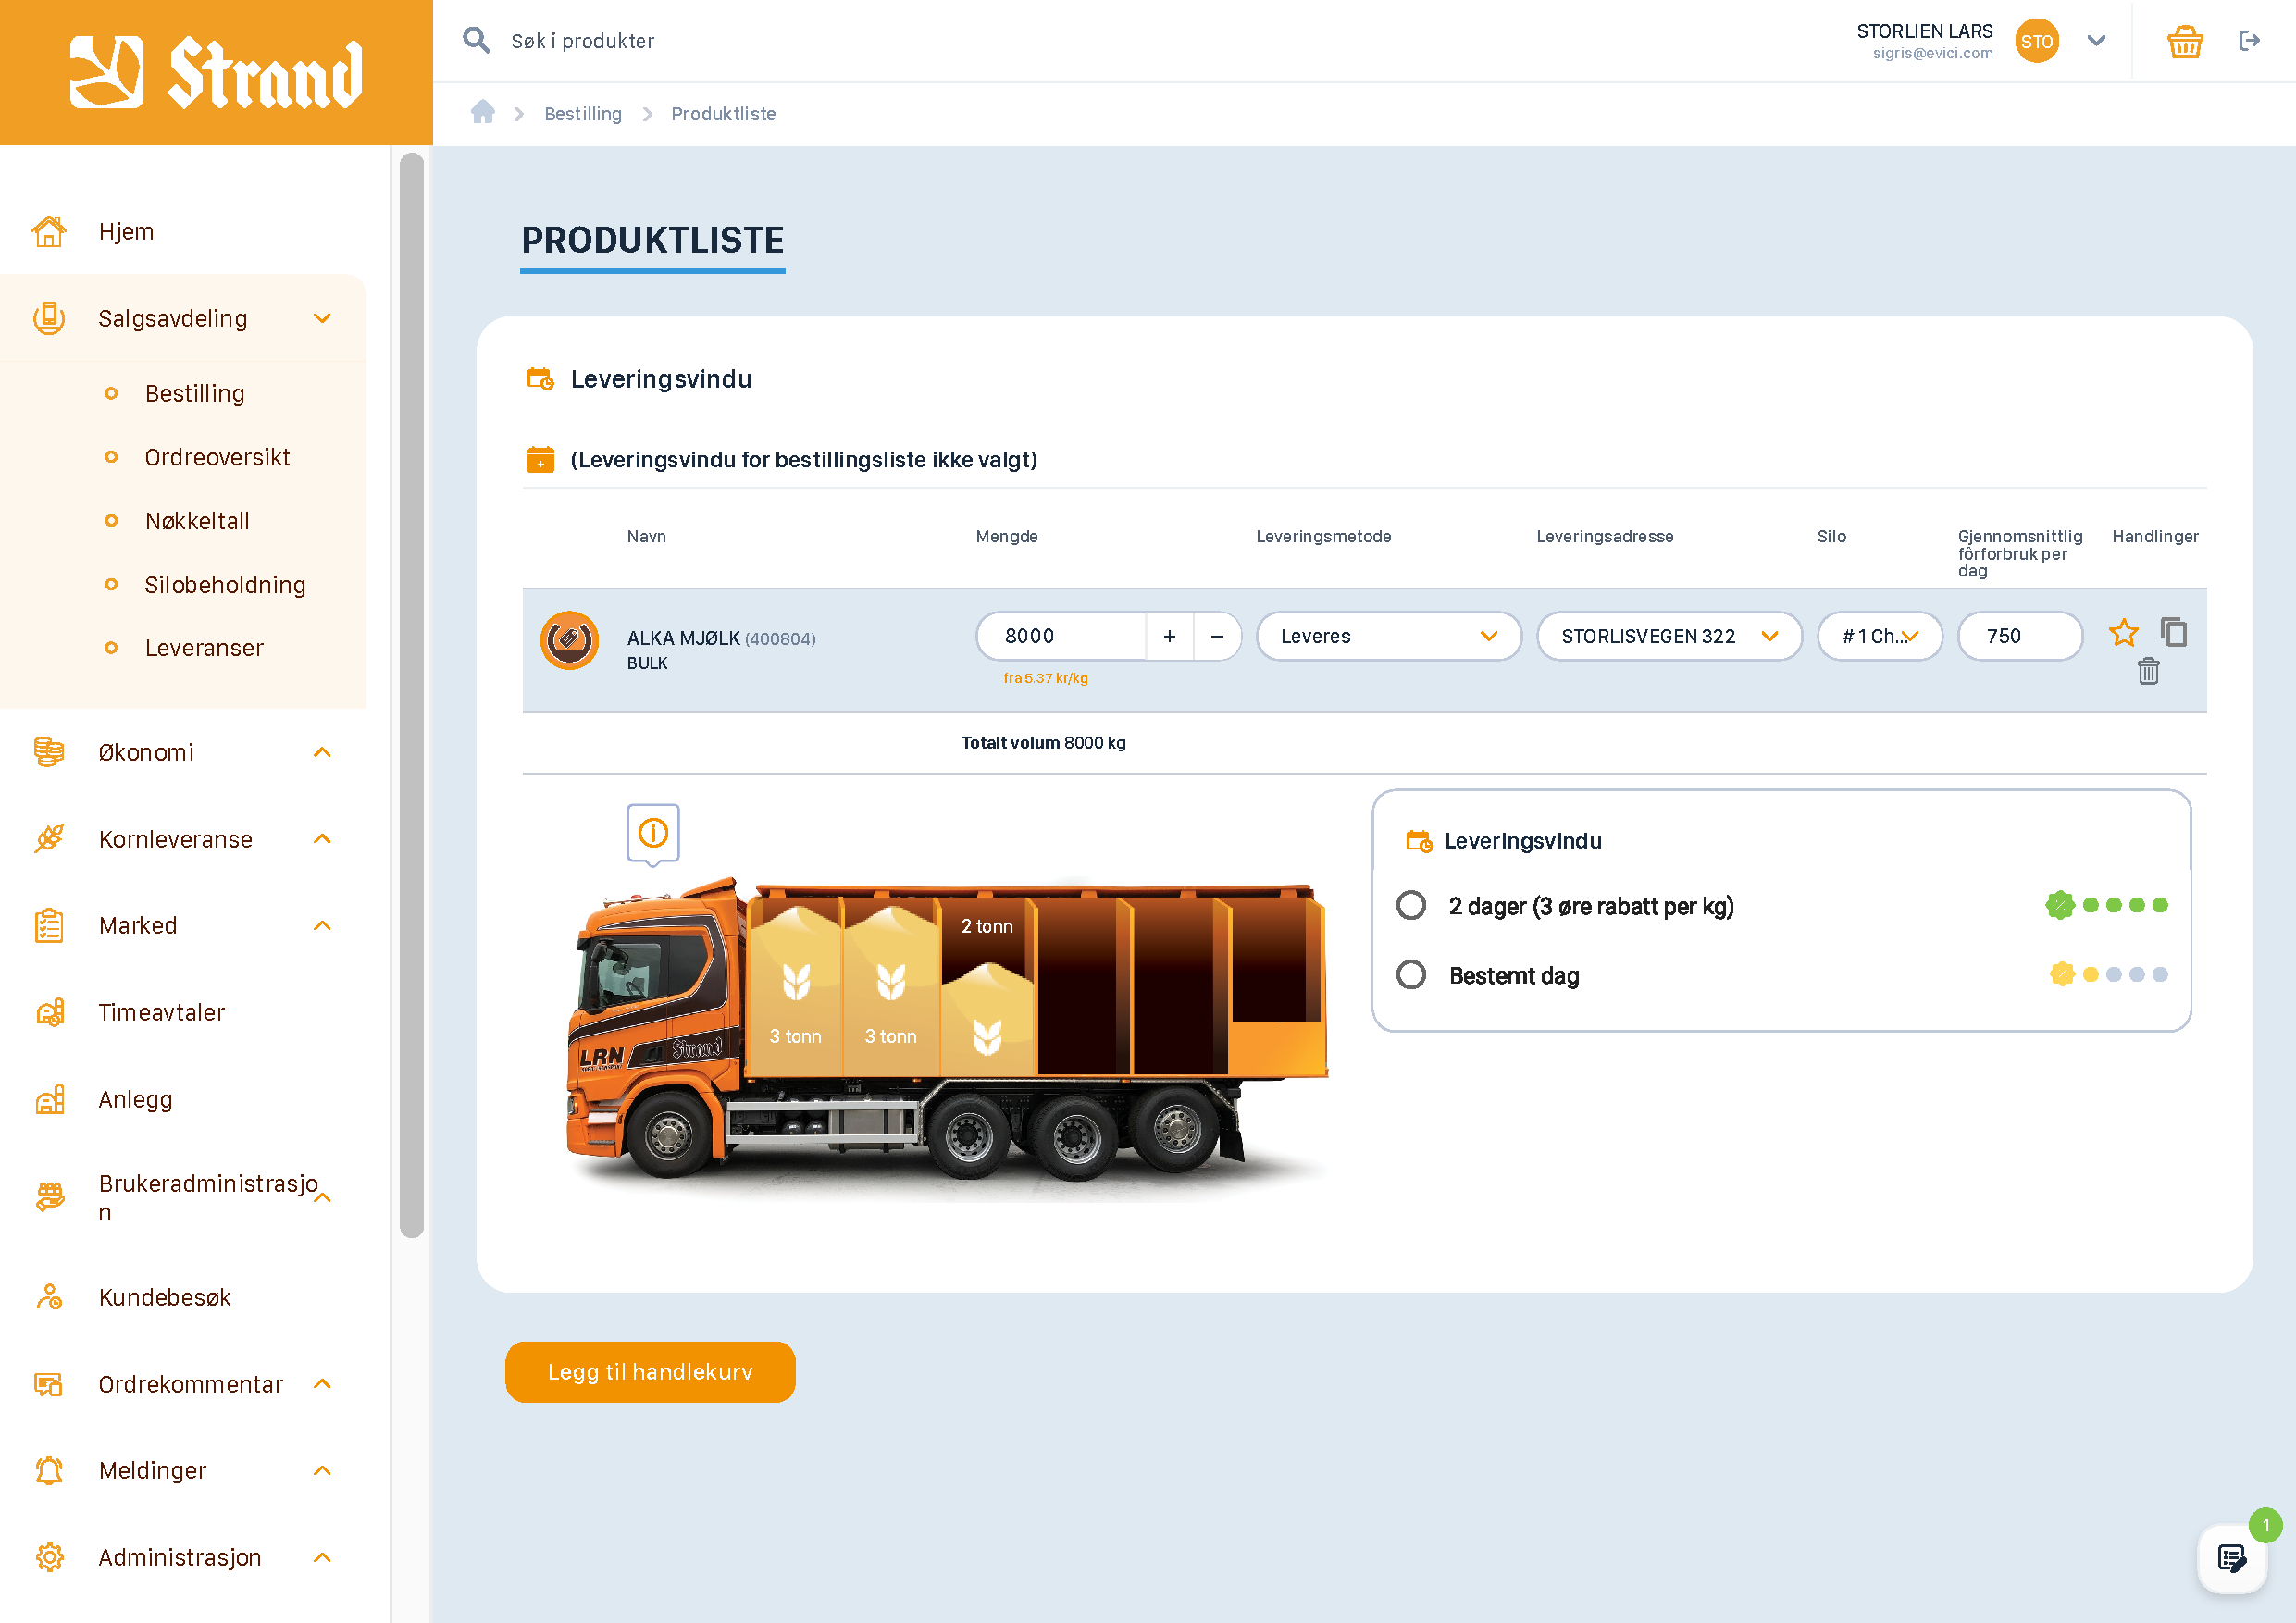
\includegraphics[width=\textwidth]{produktliste.pdf}};

  % Corner anchors for fraction-based coordinates
  \coordinate (SW) at (img.south west);
  \coordinate (SE) at (img.south east);
  \coordinate (NW) at (img.north west);

  % \ip{x}{y}: image-fraction coordinate, (0,0)=bottom-left, (1,1)=top-right.
  % Uses vector arithmetic to avoid the x-shift bug in chained ! interpolation.
  \newcommand{\ip}[2]{($(SW) + {#1}*($(SE)-(SW)$) + {#2}*($(NW)-(SW)$)$)}

  \tikzset{
    badge/.style={
      circle,
      draw=strandOrange, fill=strandOrange,
      font=\bfseries\footnotesize\sffamily, text=white,
      inner sep=1.5pt, minimum size=14pt,
      drop shadow={shadow xshift=0.5pt, shadow yshift=-0.5pt}
    },
    callout/.style={
      draw=strandOrange, fill=white,
      rounded corners=3pt,
      font=\footnotesize\sffamily,
      text=black,
      inner sep=4pt,
      align=left,
      line width=0.8pt,
      drop shadow={shadow xshift=0.5pt, shadow yshift=-0.5pt}
    },
    arrow/.style={
      -{Stealth[length=5pt]},
      color=strandOrange,
      line width=0.9pt
    }
  }

  % ---- Numbered badges with arrows to form fields ----------
  % Badge positions (offset above/beside field), arrow targets (on the field).
  % x: 0=left edge, 1=right edge  |  y: 0=bottom edge, 1=top edge

  % ---- Navigation path highlight --------------------------
  \draw[strandOrange, line width=1.5pt, rounded corners=3pt, dashed]
      \ip{0.00}{0.63} rectangle \ip{0.12}{0.84};

  % Badges 1–2: navigation steps (Salgsavdeling, Bestilling)
  \node[badge] (b1) at \ip{0.14}{0.83} {1};
  \draw[arrow] (b1) -- \ip{0.08}{0.82};   % Salgsavdeling

  \node[badge] (b2) at \ip{0.14}{0.76} {2};
  \draw[arrow] (b2) -- \ip{0.08}{0.77};   % Bestilling

  % Badges 3–7 sit above the product row, arrows point down to the fields
  \foreach \n/\bx/\tx/\ty in {
    3/0.44/0.44/0.67,
    4/0.60/0.60/0.67,
    5/0.74/0.74/0.67,
    6/0.83/0.83/0.67,
    7/0.91/0.91/0.67
  }{
    \node[badge] (b\n) at \ip{\bx}{0.79} {\n};
    \draw[arrow] (b\n) -- \ip{\tx}{\ty};
  }

  % Badge 8 sits to the right of the cart button, arrow points left
  \node[badge] (b8) at \ip{0.28}{0.04} {8};
  \draw[arrow] (b8) -- \ip{0.23}{0.04};

\end{tikzpicture}

\end{document}
